%  LaTeX support: latex@mdpi.com
%  In case you need support, please attach all files that are necessary for compiling as well as the log file, and specify the details of your LaTeX setup (which operating system and LaTeX version / tools you are using).

%=================================================================
\documentclass[water,article,submit,moreauthors,pdftex]{mdpi}

% If you would like to post an early version of this manuscript as a preprint, you may use preprint as the journal and change 'submit' to 'accept'. The document class line would be, e.g., \documentclass[preprints,article,accept,moreauthors,pdftex]{mdpi}. This is especially recommended for submission to arXiv, where line numbers should be removed before posting. For preprints.org, the editorial staff will make this change immediately prior to posting.

%% Some pieces required from the pandoc template
\setlist[itemize]{leftmargin=*,labelsep=5.8mm}
\setlist[enumerate]{leftmargin=*,labelsep=4.9mm}


%--------------------
% Class Options:
%--------------------
%----------
% journal
%----------
% Choose between the following MDPI journals:
% acoustics, actuators, addictions, admsci, aerospace, agriculture, agriengineering, agronomy, algorithms, animals, antibiotics, antibodies, antioxidants, applsci, arts, asc, asi, atmosphere, atoms, axioms, batteries, bdcc, behavsci , beverages, bioengineering, biology, biomedicines, biomimetics, biomolecules, biosensors, brainsci , buildings, cancers, carbon , catalysts, cells, ceramics, challenges, chemengineering, chemistry, chemosensors, children, cleantechnol, climate, clockssleep, cmd, coatings, colloids, computation, computers, condensedmatter, cosmetics, cryptography, crystals, dairy, data, dentistry, designs , diagnostics, diseases, diversity, drones, econometrics, economies, education, electrochem, electronics, energies, entropy, environments, epigenomes, est, fermentation, fibers, fire, fishes, fluids, foods, forecasting, forests, fractalfract, futureinternet, futurephys, galaxies, games, gastrointestdisord, gels, genealogy, genes, geohazards, geosciences, geriatrics, hazardousmatters, healthcare, heritage, highthroughput, horticulturae, humanities, hydrology, ijerph, ijfs, ijgi, ijms, ijns, ijtpp, informatics, information, infrastructures, inorganics, insects, instruments, inventions, iot, j, jcdd, jcm, jcp, jcs, jdb, jfb, jfmk, jimaging, jintelligence, jlpea, jmmp, jmse, jnt, jof, joitmc, jpm, jrfm, jsan, land, languages, laws, life, literature, logistics, lubricants, machines, magnetochemistry, make, marinedrugs, materials, mathematics, mca, medicina, medicines, medsci, membranes, metabolites, metals, microarrays, micromachines, microorganisms, minerals, modelling, molbank, molecules, mps, mti, nanomaterials, ncrna, neuroglia, nitrogen, notspecified, nutrients, ohbm, particles, pathogens, pharmaceuticals, pharmaceutics, pharmacy, philosophies, photonics, physics, plants, plasma, polymers, polysaccharides, preprints , proceedings, processes, proteomes, psych, publications, quantumrep, quaternary, qubs, reactions, recycling, religions, remotesensing, reports, resources, risks, robotics, safety, sci, scipharm, sensors, separations, sexes, signals, sinusitis, smartcities, sna, societies, socsci, soilsystems, sports, standards, stats, surfaces, surgeries, sustainability, symmetry, systems, technologies, test, toxics, toxins, tropicalmed, universe, urbansci, vaccines, vehicles, vetsci, vibration, viruses, vision, water, wem, wevj

%---------
% article
%---------
% The default type of manuscript is "article", but can be replaced by:
% abstract, addendum, article, benchmark, book, bookreview, briefreport, casereport, changes, comment, commentary, communication, conceptpaper, conferenceproceedings, correction, conferencereport, expressionofconcern, extendedabstract, meetingreport, creative, datadescriptor, discussion, editorial, essay, erratum, hypothesis, interestingimages, letter, meetingreport, newbookreceived, obituary, opinion, projectreport, reply, retraction, review, perspective, protocol, shortnote, supfile, technicalnote, viewpoint
% supfile = supplementary materials

%----------
% submit
%----------
% The class option "submit" will be changed to "accept" by the Editorial Office when the paper is accepted. This will only make changes to the frontpage (e.g., the logo of the journal will get visible), the headings, and the copyright information. Also, line numbering will be removed. Journal info and pagination for accepted papers will also be assigned by the Editorial Office.

%------------------
% moreauthors
%------------------
% If there is only one author the class option oneauthor should be used. Otherwise use the class option moreauthors.

%---------
% pdftex
%---------
% The option pdftex is for use with pdfLaTeX. If eps figures are used, remove the option pdftex and use LaTeX and dvi2pdf.

%=================================================================
\firstpage{1}
\makeatletter
\setcounter{page}{\@firstpage}
\makeatother
\pubvolume{xx}
\issuenum{1}
\articlenumber{5}
\pubyear{2019}
\copyrightyear{2019}
%\externaleditor{Academic Editor: name}
\history{Received: date; Accepted: date; Published: date}
\updates{yes} % If there is an update available, un-comment this line

%% MDPI internal command: uncomment if new journal that already uses continuous page numbers
%\continuouspages{yes}

%------------------------------------------------------------------
% The following line should be uncommented if the LaTeX file is uploaded to arXiv.org
%\pdfoutput=1

%=================================================================
% Add packages and commands here. The following packages are loaded in our class file: fontenc, calc, indentfirst, fancyhdr, graphicx, lastpage, ifthen, lineno, float, amsmath, setspace, enumitem, mathpazo, booktabs, titlesec, etoolbox, amsthm, hyphenat, natbib, hyperref, footmisc, geometry, caption, url, mdframed, tabto, soul, multirow, microtype, tikz

%=================================================================
%% Please use the following mathematics environments: Theorem, Lemma, Corollary, Proposition, Characterization, Property, Problem, Example, ExamplesandDefinitions, Hypothesis, Remark, Definition
%% For proofs, please use the proof environment (the amsthm package is loaded by the MDPI class).

%=================================================================
% Full title of the paper (Capitalized)
\Title{Analysis of Access to Emergency Funds in Sub-Saharan Countries--
A Human Rights-Based Approach}

% Authors, for the paper (add full first names)
\Author{Rose
Porta$^{1,\ddagger,*}$\href{https://orcid.org/0000-0001-7296-6830}{\orcidicon}, Alejandra
Munoz
Garcia$^{1,\ddagger}$\href{https://orcid.org/0000-0002-9687-2342}{\orcidicon}, Margaret
Bassney$^{1,\ddagger}$\href{https://orcid.org/0000-0003-2843-6271}{\orcidicon}, Aushanae
Haller$^{1,\ddagger}$\href{https://orcid.org/0000-0002-2090-1952}{\orcidicon}}

% Authors, for metadata in PDF
\AuthorNames{Rose Porta, Alejandra Munoz Garcia, Margaret
Bassney, Aushanae Haller}

% Affiliations / Addresses (Add [1] after \address if there is only one affiliation.)
\address{%
$^{1}$ \quad Department of Statistical and Data Sciences, Smith College,
Northampton MA; \\
}
% Contact information of the corresponding author
\corres{Correspondence: \href{mailto:rporta@smith.edu}{\nolinkurl{rporta@smith.edu}}}

% Current address and/or shared authorship
\firstnote{These authors contributed equally to this work.}







% The commands \thirdnote{} till \eighthnote{} are available for further notes

% Simple summary

% Abstract (Do not insert blank lines, i.e. \\)
\abstract{Most people require access to emergency funds at least once in
their life. These funds act as an important safety net in emergency
cases. The purpose of our project is to predict access to emergency
funds for adults in Sub-Saharan countries using a human rights-based
approach to machine learning which centers equity, fairness, and impacts
on humans over accuracy. Our analysis is based on the 2017 Global Findex
Database which includes demographic as well as financial information for
a sample of individuals within each country. We used a Decision Tree
Classifier machine learning model implemented using Python to predict
access to emergency funds with 68\% accuracy. We assessed the fairness
of our model with respect to gender using a variety of group and
individual fairness metrics and evaluated the implications of each
fairness metric with regard to our data and the goals of the analysis.
We then implemented a variety of pre-proccessing, in-processing, and
post-processing techniques in an attempt to minimize bias and maximize
fairness. We have documented our analysis in a Jupyter notebook where
this information can be made accessible to a broader undergraduate
audience.}

% Keywords
\keyword{Fairness; machine learning; access; emergency funds; financial;
ethics; processing techniques; gender; economy; debiasing; decision
tree; Sub-Saharan Africa; fairness metrics}

% The fields PACS, MSC, and JEL may be left empty or commented out if not applicable
%\PACS{J0101}
%\MSC{}
%\JEL{}

%%%%%%%%%%%%%%%%%%%%%%%%%%%%%%%%%%%%%%%%%%
% Only for the journal Diversity
%\LSID{\url{http://}}

%%%%%%%%%%%%%%%%%%%%%%%%%%%%%%%%%%%%%%%%%%
% Only for the journal Applied Sciences:
%\featuredapplication{Authors are encouraged to provide a concise description of the specific application or a potential application of the work. This section is not mandatory.}
%%%%%%%%%%%%%%%%%%%%%%%%%%%%%%%%%%%%%%%%%%

%%%%%%%%%%%%%%%%%%%%%%%%%%%%%%%%%%%%%%%%%%
% Only for the journal Data:
%\dataset{DOI number or link to the deposited data set in cases where the data set is published or set to be published separately. If the data set is submitted and will be published as a supplement to this paper in the journal Data, this field will be filled by the editors of the journal. In this case, please make sure to submit the data set as a supplement when entering your manuscript into our manuscript editorial system.}

%\datasetlicense{license under which the data set is made available (CC0, CC-BY, CC-BY-SA, CC-BY-NC, etc.)}

%%%%%%%%%%%%%%%%%%%%%%%%%%%%%%%%%%%%%%%%%%
% Only for the journal Toxins
%\keycontribution{The breakthroughs or highlights of the manuscript. Authors can write one or two sentences to describe the most important part of the paper.}

%\setcounter{secnumdepth}{4}
%%%%%%%%%%%%%%%%%%%%%%%%%%%%%%%%%%%%%%%%%%


% tightlist command for lists without linebreak
\providecommand{\tightlist}{%
  \setlength{\itemsep}{0pt}\setlength{\parskip}{0pt}}




\begin{document}


%%%%%%%%%%%%%%%%%%%%%%%%%%%%%%%%%%%%%%%%%%

\hypertarget{introduction}{%
\section{Introduction}\label{introduction}}

Science is often viewed as a way to offer trustworthy research backed
solutions and answers. A lot of that research involves statistical
methods performed on data. However, what happens when the data and
statistical methods are not objective and trustworthy as is so often
assumed? The conclusions drawn from the data are biased and unfair, most
often towards minorities and protected classes of people. In order
ensure that the outcomes of our analysis are equitable and positively
impactful, our goal is to establish a human rights-based approach to
machine learning analysis. A human right-based approach is characterized
by awareness of context and consideration of the impacts the outcomes
will have on humans through each stage of the data analysis process.
More concretely, this process looks like (1) researching the context of
the dataset before beginning any analysis; (2) performing exploratory
data analysis to bring awareness to imbalances and relationships that
exist in the data; (3) thoughtfully choosing an appropriate model based
on the context of the data; (4) implementing fairness metrics to assess
bias in the model; and (5) implementing de-biasing techniques to improve
fairness.

We use a World Bank Global Findex data set which contains financial
information about 35 Sub Saharan countries. Specifically, we create a
model to predict access to emergency funds, defined as 1/20th of the GNI
(gross national income) per capita for the country, then analyze the
fairness of the model. We focus on group and individual fairness metrics
for the protected attribute sex. In addition we investigate the data set
itself to understand where potential biases might have been implanted.

Data sets and algorithms have real world impacts on real people. The
inherent bias in data sets can carry over into machine learning
algorithms that are used to profile and categorize people
\citep{navarro2021risk, hellstrom2020bias}. Since data sets are not
collected in a vacuum and often represent the discriminatory
environments in which they are collected
\citep{barocas_fairness_nodate}, we must find ways to make data sets and
statistical methods more equitable. In this study we explore fairness
methods that can be used to evaluate machine learning models. The
``impossibility theorem'' is the idea that not all fairness metrics can
be satisfied at the same time \citep{kleinberg2016inherent}. Although
fairness is complex and there are multiple approaches to make a model
fair \citep{kypraiou_what_2021, green2018myth}, it is important to
continue to question how data and algorithms can be biased and how to
mitigate that bias.

While there have been previous studies implementing fairness techniques
in different contexts \citep{deho2022existing, kim2022information}, we
implement them in an exploratory context meant to teach how and when to
use these techniques thus giving us more freedom to branch beyond a
specific question while supporting previous work about the importance of
these fairness metrics
\citep{anahideh2022fair, barocas_fairness_nodate}. We analyse the data,
data collection methods, prediction models, and the fairness metrics to
assess how biased our data is and understand how we can de-bias when
possible.

This approach will be used as the basis of a workshop meant to educate
data science and computer science students on how to integrate ethics
and fairness into their machine learning workflows. The analysis
outlined in this paper is meant to serve as an example of an
implementation of a human rights-based approach to machine learning.
Thus, we focus more on explaining the process as it applies to this
analysis more than the results of the analysis itself.

\hypertarget{data}{%
\section{Data}\label{data}}

Our data is derived from The World Bank in The Global Findex Database,
comprising the most comprehensive data sets on how adults save, borrow,
make payments, and manage risk in different economies around the world.
The data set was created to record various measures of financial equity
and inclusion, with the intention that such information could reveal
opportunities to expand access to financial services and to promote
greater use of digital financial services for individuals who do not
have a bank account.

The survey was carried out over the 2017 calendar year by Gallup, Inc.,
as part of its Gallup World Poll, which since 2005 has annually
conducted surveys of approximately 1,000 people in each of more than 160
economies and in over 150 languages, using randomly selected, nationally
representative samples. The target population was the entire civilian,
noninstitutionalized population age 15 and above. Interview procedure
Surveys were conducted face to face in economies where telephone
coverage represents less than 80 percent of the population or where this
was the customary methodology.

In economies where face-to-face surveys were conducted, the first stage
of sampling was the identification of primary sampling units. These
units were stratified by population size, geography, or both, and
clustering was achieved through one or more stages of sampling. Where
population information was available, sample selection was based on
probabilities proportional to population size; otherwise, simple random
sampling was used. Random route procedures were used to select sampled
households. Unless an outright refusal occurs, interviewers make up to
three attempts to survey the sampled household. If an interview cannot
be obtained at the initial sampled household, a simple substitution
method was used.

Respondents were randomly selected within the selected households. Each
eligible household member was listed and the handheld survey device
randomly selects the household member to be interviewed. For paper
surveys, the Kish grid method was used to select the respondent. In
economies where cultural restrictions dictate gender matching,
respondents were randomly selected from among all eligible adults of the
interviewer's gender.

In economies where telephone interviewing was employed, random digit
dialing or a nationally representative list of phone numbers was used.
In most economies where cell phone penetration was high, a dual sampling
frame was used. Random selection of respondents was achieved by using
either the latest birthday or household enumeration method.

There were several variables of interest in this dataset when creating
models to predict access to emergency funds, including demographic and
financial information. For this analysis, we are using only a subset of
the data including countries in the Sub-Saharan region (35 countries
total). Our data set includes 35000 observations and 105 variables in
total.

\hypertarget{demographics}{%
\subsection{Demographics}\label{demographics}}

\hypertarget{gender}{%
\subsubsection{\texorpdfstring{\emph{gender}}{gender}}\label{gender}}

The variable \emph{gender} distinguishes gender. There are 17,870
females and 17,130 males in the dataset.

\hypertarget{education}{%
\subsubsection{\texorpdfstring{\emph{Education}}{Education}}\label{education}}

The \emph{Education} variable corresponds to the highest level of
education attained with `Primary', `Secondary' and `Tertiary' being the
three options. The distribution of education by gender plot (seen in
Appendix Figure 8) shows us that there are more women with primary
education, but more men with secondary or tertiary education. Overall,
we can see that there are more men with higher education than women.
About 1,000 more men have received a secondary education and there is
about double the amount of men with tertiary education compared to women
showing a clear disparity.

\hypertarget{economy}{%
\subsubsection{\texorpdfstring{\emph{economy}}{economy}}\label{economy}}

The final demographic variable of interest is the \emph{economy}
variable that separates respondents by which country they live in. There
are 35 different countries from Sub-Saharan Africa with exactly 1000
respondents from each. The countries included are Benin, Botswana,
Burkina Faso, Cameroon, Central African Republic, Chad, Congo, Dem.
Rep., Congo, Rep., Cote d'Ivoire, Ethiopia, Gabon, Ghana, Guinea, Kenya,
Lesotho, Liberia, Madagascar, Malawi, Mali, Mauritania, Mauritius,
Mozambique, Namibia, Niger, Nigeria, Rwanda, Senegal, Sierra Leone,
South Africa, South Sudan, Tanzania, Togo, Uganda, Zambia, and Zimbabwe.

\hypertarget{financial}{%
\subsection{Financial}\label{financial}}

In the following, we will take a closer look at financial related
variables that seem likely to have an impact to the access to emergency
funds.

\hypertarget{account_fin}{%
\subsubsection{\texorpdfstring{\emph{account\_fin}}{account\_fin}}\label{account_fin}}

The first variable being \emph{account\_fin} which distinguishes those
who have a financial account from those who don't. We found 11,970
respondents have a financial account while 23,030 respondents do not.
This means about two thirds of individuals do not have an account. This
is likely connected to the lack of access to emergency funds displayed
above. If an individual does not have a financial account, we would
expect they are less likely to have a source of emergency funds, as
emergency funds are generally stored in an account.

\hypertarget{reason}{%
\subsubsection{\texorpdfstring{\emph{reason}}{reason}}\label{reason}}

Those who do not have a financial account were asked why in the
\emph{reason} variable, that provides a list of possible reasons for not
having a financial account (seen in Appendix Figure 9).

\hypertarget{emp_in}{%
\subsubsection{\texorpdfstring{\emph{emp\_in}}{emp\_in}}\label{emp_in}}

Employment status was another financial variable of interest represented
by \emph{emp\_in}, which asks whether or not the participant is in the
workforce. It appears that 10,715 individuals were not in the workforce
while 24.285 were, meaning about three-fourths of individuals are in the
workforce.

\hypertarget{inc_q}{%
\subsubsection{\texorpdfstring{\emph{inc\_q}}{inc\_q}}\label{inc_q}}

And lastly, we evaluated \emph{inc\_q}, which represents income
quantile. Income quantile is separated into 5 quantiles with 1 being the
poorest and 5 being the richest. The mean for all of the countries in
the dataset is 3.241. This means that all the countries average out to
be about middle class.

The majority of the data set has individuals within the richest
quantile, Quantile 5.

\hypertarget{emergency-funds}{%
\subsection{Emergency Funds}\label{emergency-funds}}

To explore access to emergency funds in our dataset, we were interested
3 variables we thought could be related:

\hypertarget{has_access}{%
\subsubsection{\texorpdfstring{\emph{has\_access}}{has\_access}}\label{has_access}}

The variable \emph{has\_access} directly asks participants if they have
access to emergency funds, with ``emergency funds'' defined as 1/20th of
the GNI (gross national income) per capita for the country. GNI per
capita is the country's total income in a year/ the country's population
size. For context, in the United States, ``emergency funds'' would be
defined as about \$3,000.

The overall distribution of access to emergency funds showed 15,237
individuals had access to emergency funds while 18,867 did not. This
indicates that over half of individuals represented in the data do not
have access.

\hypertarget{main_source_funds}{%
\subsubsection{\texorpdfstring{\emph{main\_source\_funds}}{main\_source\_funds}}\label{main_source_funds}}

We proceeded to explore the source of emergency funds using the
\emph{main\_source\_funds} variable, which provides a list of options
for where participants receive their main source of emergency funds:

\begin{figure}
\centering
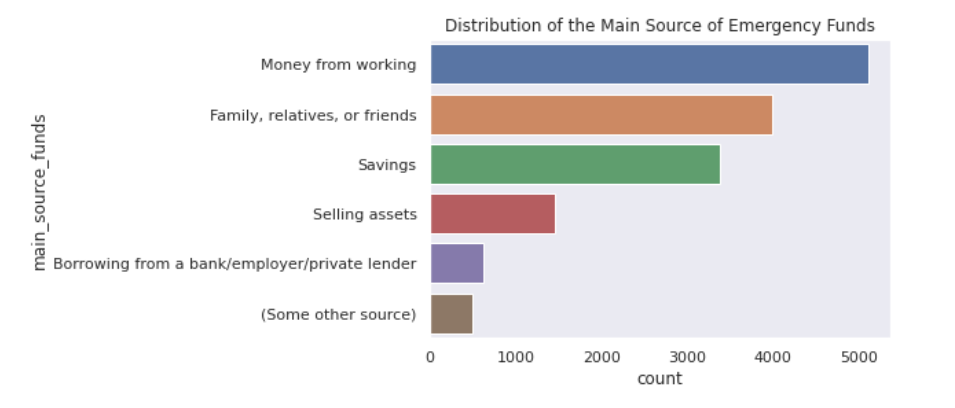
\includegraphics[width=\textwidth,height=0.5\textheight]{images/MainSourceFunds.png}
\caption{Distribution of Main Source of Emergency Funds}
\end{figure}

Figure 1 displays the overall distribution of the main source of
emergency funds. Most of the individuals with access to emergency funds
receive their funding from work, their family and friends, or their
savings.

\hypertarget{receive-wage-payments}{%
\subsubsection{\texorpdfstring{\emph{Receive Wage
Payments}}{Receive Wage Payments}}\label{receive-wage-payments}}

If respondents answered that their main source of emergency funds was
from `Money From Working', they were asked to further clarify the form
in which that money was received. From that ``Money from Working''
category, we can see that only 8,348 individuals receive wage payments
from the \emph{Receive Wage Payments} variable while 26,241 do not. This
analysis suggests that receiving wage payments may be a key factor in
determining access to emergency funds.

\hypertarget{gender-economy-and-education-in-relation-to-emergency-funds}{%
\subsubsection{\texorpdfstring{\emph{gender}, \emph{economy} and
\emph{Education} in relation to Emergency
Funds}{gender, economy and Education in relation to Emergency Funds}}\label{gender-economy-and-education-in-relation-to-emergency-funds}}

Finally, we sought to find if there were disparities in access to
emergency funds by \emph{gender}, \emph{economy}, and \emph{Education}.

\begin{figure}
\centering
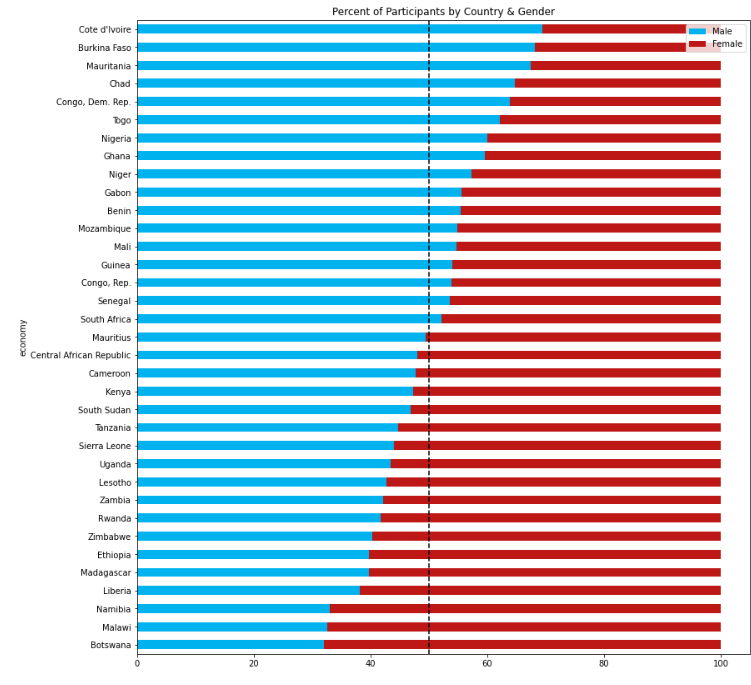
\includegraphics[width=\textwidth,height=0.5\textheight]{images/percent_participants_by_country_gender.png}
\caption{Percent of Participants by Country \& Gender}
\end{figure}

\begin{figure}
\centering
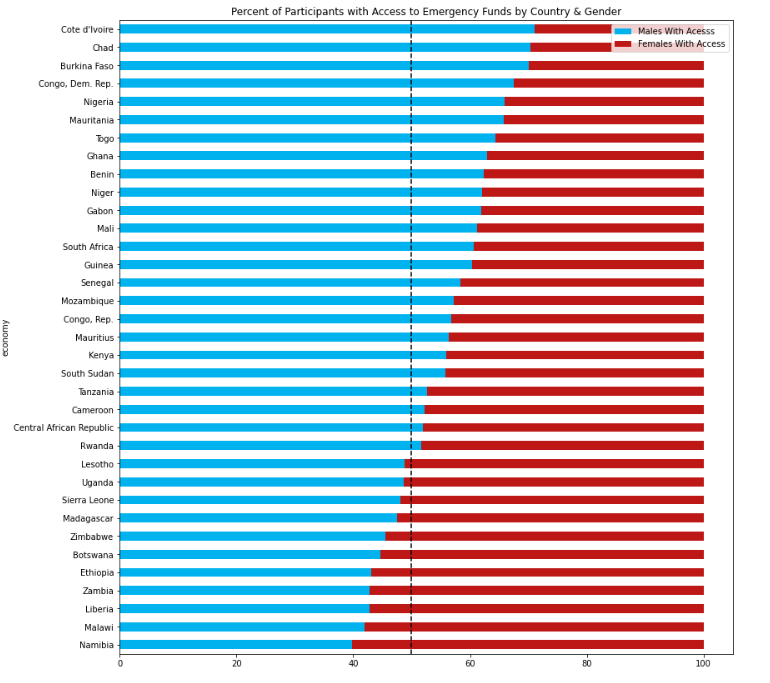
\includegraphics[width=\textwidth,height=0.5\textheight]{images/percent_access_funds_by_country_gender.png}
\caption{Percent of Participants with Access to Emergency Funds by
Country \& Gender}
\end{figure}

In the side-by-side barplots shown in figures 2 and 3, we can see that
although only about 50\% of the countries have a higher percentage of
men represented in the questionnaire (left bar plot), in 75\% of the
countries more men have access to emergency funds than women (right bar
plot).

\begin{figure}
\centering
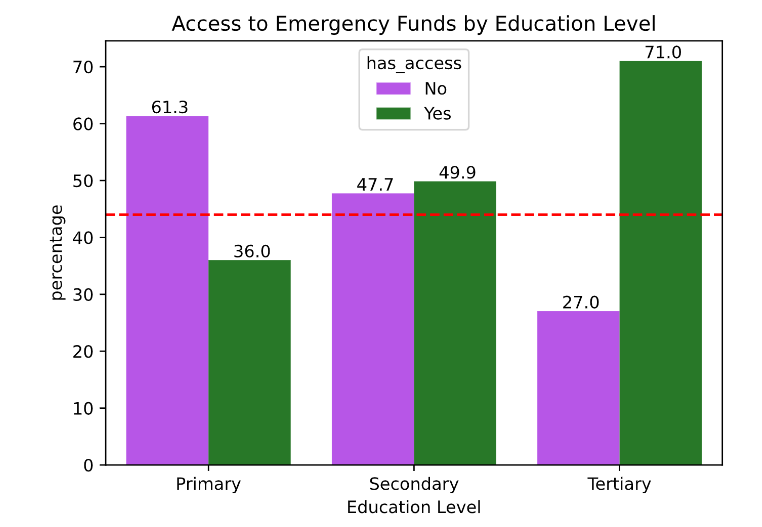
\includegraphics[width=\textwidth,height=0.5\textheight]{images/access_by_educ_level.png}
\caption{Access to Emergency Funds by Education Level}
\end{figure}

Additionally, in figure 4, we can see the distribution of funds based on
an individual's highest education level. 63\% of people with only a
primary education do not have access to emergency funds compared to 37\%
of people who do. These numbers are more evenly distributed for those
with secondary education, with about 49\% of people not having access to
emergency funds, while 51\% of people do have access. Finally, for those
with a tertiary level of education we can see that about 72\% of people
have access to emergency funds while only 28\% of that group does not
have access. Overall, we can make the assumption that people with a
higher level of education are more likely to have access to emergency
funds.

\hypertarget{methods}{%
\section{Methods}\label{methods}}

\hypertarget{software}{%
\subsection{Software}\label{software}}

We conducted our analysis in a Google Colab Notebook primarily employing
the python libraries \href{https://pandas.pydata.org/}{pandas} and
\href{https://numpy.org/}{numpy} for data cleaning and exploratory
analysis, as well as \href{https://scikit-learn.org/stable/}{sklearn}
and \href{https://aif360.readthedocs.io/en/latest/}{aif360} for
implementing machine learning methods, fairness metrics, and de-biasing
techniques. The notebook detailing our
\href{https://github.com/sds-capstone/2022-09-proj7-women-at-table/blob/main/final_project.ipynb}{full
analysis} is available via our public
\href{https://github.com/sds-capstone/2022-09-proj7-women-at-table}{GitHub
repository}.

\hypertarget{data-cleaning}{%
\subsection{Data Cleaning}\label{data-cleaning}}

Before fitting the model, we performed several pre-processing steps on
the data in order to remove unnecessary or redundant information,
address missing values, and ensure that the variables were coded such
that they would be processed appropriately by the model. Some of these
steps were performed after fitting the initial model, and some choices
were made based on the impacts of those choices on the performance of
the model.

First, we removed the arbitrary variables \emph{economycode} (country
code) and \emph{regionwb} (region); \emph{economycode} is essentially a
duplicate of \emph{economy} (country name), and \emph{regionwb} is the
same for all rows (value is Sub-Saharan) since this is the variable that
we initially filtered by. Next, we checked for variables with a high
percentage of missing values. Several variables have many missing values
because they are follow-up questions to a previous question that are
only asked if the respondent gives a specific response for a previous
question. We chose to drop all variables with more than 30\% missing
values (58 variables total) because we observed by running the model
multiple times that variables with NA percentages above this threshold
had no impact on the model accuracy or fairness. Thus, it made sense to
remove them if their presence is negligible when included in the model.
Next, we checked for variables with high levels of redundancy
(i.e.~little variation), defining a high level of redundancy as 95\% or
more of the values being the same. The only variable with a high level
of redundancy was \emph{pay\_online} (a binary variable indicating
whether or not an individual has paid online for something), and we
chose to remove it because removing it had no impact on the model
accuracy and fairness.

The most common answer format of the survey was multiple choice with
answer options ``yes'', ``no'', ``don't know'', and ``refuse''. Based on
our exploratory data analysis, it seems that for most questions, the
numbers of ``don't know'' and ``refuse'' responses are very low.
Furthermore, these responses would not give us much useful information
when implementing a predictive model. Thus, we chose to replace all
``don't know'' and ``refuse'' values with \emph{NA} values. We then
replaced all remaining missing values (including missing values not
removed previously and ``don't know'' and ``refuse'' values) with the
column mean rounded to the nearest whole number (i.e.~the most frequent
value if the variable is categorical).

Next, we re-coded the country variable into a variable with five
categories based on the percentage of sampled individuals in the country
who have access to emergency funds (1 = \textless{} 20\% have access, 2
= between 20\% and 40\% have access, etc.). All other variables in our
data set were coded such that the model could appropriately interpret
them, so we did not have to do any additional re-coding. The majority of
the variables are binary with 0 = no, 1 = yes, and the rest are either
categorical variables with hierarchical categories such as income
quantile and education level or continuous numerical variables such as
age.

Finally, we created a cartesian product to combine two variables -- one
indicating whether or not an individual has a financial account and the
other indicating whether or not the individual has saved money in the
past 12 months-- in order to increase the accuracy of the model after
fitting the initial model.

After this pre-processing, we have 42 predictor variables and 35,000
observations.

\hypertarget{model-selection}{%
\subsection{Model Selection}\label{model-selection}}

Given that we are aiming to predict a binary outcome (possible or not
possible to come up with emergency funds), our model needs to be a
classification model. We tried two of the most common model types used
for classification-- logistic regression and decision tree classifier.
We ultimately chose the decision tree classifier model over the logistic
regression model because the baseline accuracy was higher (61\% versus
55\%). Furthermore, the decision tree model makes more intuitive sense
given our data since most of our predictors are binary variables, and
binary predictors fit well into the tree structure. We were able to
further improve the accuracy of the decision tree model to 68\% by using
cross-validation to specify the max depth as 6. The decision tree model
uses machine learning to predict outcomes by organizing the variables
into a tree that branches off at each decision point based on the value
of the variable at that point. The most influential variables are at the
top, and the outcome variable is at the end of each branch. We split our
data into 70\% training, 30\% testing because this is the standard
train-test split used for machine learning algorithms.

\hypertarget{metrics}{%
\subsection{Metrics}\label{metrics}}

To assess fairness and accuracy in our model we explore 12 different
metrics, 10 of which are fairness metrics. Fairness metrics can be split
into group and individual metrics.

\hypertarget{basic-metrics}{%
\subsubsection{Basic Metrics}\label{basic-metrics}}

\hypertarget{accuracy.}{%
\paragraph{Accuracy.}\label{accuracy.}}

Accuracy is a measure of how many classifications our model predicts
correctly compared to all the predictions. The ratio of correctly
predicted classifications to all the predictions. Accuracy cannot tell
us if the predictions are equally correct across positives and negatives
\citep{juba2019precision, gupta2021recall}. 55\% of the people in our
data set don't have access to emergency funds. As long as our model
predicts negatives more than half the time, we can get a good accuracy.
However, our model will lose the ability to accurately predict
positives. It is important to consider accuracy along with precision and
recall so we can more fully understand how our model is classifying
people.

\(Accuracy = (True Positives + True Negatives) / (True Positives + True Negatives + False Positives + False Negatives)\)

\hypertarget{precision.}{%
\paragraph{Precision.}\label{precision.}}

Precision is a measure of how accurately a model predicts positive
outcomes.The ratio of correctly predicted positives to all predicted
positives. With high precision rates, we have low false positive rates
\citep{juba2019precision, gupta2021recall}.

\(Precision = true positives / (true positives + false positives)\)

\hypertarget{recall.}{%
\paragraph{Recall.}\label{recall.}}

Recall is a measure of how accurately a model predicts negative
outcomes.The ratio of correctly predicted negatives to all predicted
negatives\citep{gupta2021recall}

\(Recall = true negatives / all negatives)\)

\hypertarget{fairness-metrics}{%
\subsubsection{Fairness Metrics}\label{fairness-metrics}}

Fairness metrics are a way to assess machine learning algorithms for
unwanted bias. Algorithms can classify people unfairly using data
collected in a biased environment. When classifying people, it is
important to take into account how these classifications can contribute
to and reinforce discriminatory social systems. Thus, it is sometimes
necessary to sacrifice accuracy in favor of fairness when using machine
learning algorithms to make decisions impacting people
\citep[\citet{kamiran2012data},
\citet{menon2018cost}]{zliobaite2015relation}. It is often not possible
to maximize fairness and accuracy at the same time because due to
discriminatory systems built into society, protected attributes such as
gender are often associated with the outcome variable. With regard to
our dataset, the proportion females with access to emergency funds is
substantially lower that that for men in the sample. Because of this,
the model will be less likely to predict positive values for females. If
the model were to hypothetically be used to determine which individuals
to offer loans to, it would reinforce existing patriarchal systems to
offer fewer loans to females. Thus, it would be beneficial to prioritize
equitable access to loans by gender over accuracy. In other words,
reality is often not fair, so if we only prioritize accuracy, we will
continue to replicate the discriminatory systems that exist.

One approach to fairness in machine learning is ``fairness by
unawareness'' meaning a model is blind to the sensitive attributs.
Although it may seem an intuitive approach to simply remove the
protected attribute from the data in order to make the algorithm
unbiased, this is often not an effective approach to reduce bias. There
are often variables that remain in the data that act as pseudo
substitutes for the protected attribute \citep{zhou2022bias}. For
example, if race was excluded from the model but the variable zip code
remained. Zip code can act as a stand in for race in regions where
people are segregated by race. Another concrete example of this is the
amazon recruiter tool removed gender from their algorithm but it was
still biased against women \citep{goodman_2022}.

In our case we are focusing on the protected attribute gender. If we
were to remove the gender variable from our data, it is possible that
our model could still have gender bias given that there are other
variables in the dataset that have a strong association with gender
including education and several of the finanical variables (as shown in
our exploratory data analysis).

\hypertarget{individual-fairness-metrics}{%
\paragraph{Individual Fairness
Metrics}\label{individual-fairness-metrics}}

Individual fairness metrics measure how similarly the model predicts for
similar observations. Will two very similar people receive the same
classification? Individual fairness metrics contradict group fairness
metrics. When accounting for imbalanced predictions between groups, the
within group fairness can suffer\citep{kypraiou_what_2021}. In the
process of satisfying group metrics, two similar subjects only differing
by sex, may be classified differently
\citep{binns2020apparent, mehrabi2021survey, caton2020fairness, zhou2022bias}.
The individual metrics we explore are general entropy error and
consistency score. We can measure both individual and group fairness
with the between group general entropy error metric.

\hypertarget{general-entropy-error.}{%
\subparagraph{General Entropy Error.}\label{general-entropy-error.}}

This metric is an individual metric, and it computes fairness by
computing the level of unfair benefit being assigned by the model. The
metric defines ``benefit'' as follows: for any individual in the testing
data set, that individual has received a benefit if the model predicted
the favorable outcome when the truth was that the individual did not
have the favorable outcome (i.e.~a false positive). Each individual in
the data receives either a 2 (benefit, false positive), a 1 (no benefit,
correct prediction), or 0 (no benefit, false negative). The metric then
compares the benefit of each individual to the average accuracy and
false positive level of the model. The ``ideal'' value is 0, and a
higher number indicates a higher level of inequity in benefit among
individuals. In other words, if many individuals have a benefit score
that is far off from the average, that indicates that the model is
unfairly benefiting some individuals and not others. This metric does
not consider privileged versus unprivileged groups, and thus is not able
to indicate whether or not the inequality in benefit is systematic in
any particular way (i.e., it cannot tell whether males receive more
benefit than females; it can only tell that some individuals receive
higher benefits than others)
\citep{caton2020fairness, kypraiou_what_2021}.

This metric is important to our data because a false positive
outcome(higher benefit) would mean that someone is predicted to having
access to emergency funds when they don't. If there is a high general
entropy error, there are many individuals whose need for emergency funds
are being overlooked.

\hypertarget{group-fairness-metrics}{%
\paragraph{Group Fairness Metrics}\label{group-fairness-metrics}}

Group fairness metrics ensure parity between privileged and unprivileged
groups of a protected class. For example, for the protected class sex,
the privileged group is men and the unprivileged group is women. The
model should work similarly for both of these groups and not favor the
privileged group. Group fairness metrics measures how discriminatory the
model classifies the unprivileged
group\citep{binns2020apparent, mehrabi2021survey, caton2020fairness}.
The group metrics we explore include statistical parity difference,
equal opportunity difference, disparate impact,precision score
difference, general entropy difference,and conditional demographic
parity.Not all group fairness metrics can be satisfied at the same time.
For example equal opportunity difference and statistical parity
difference cannot be simultaneously accounted
for\citep{kypraiou_what_2021}.

\hypertarget{statistical-parity-difference.}{%
\subparagraph{Statistical Parity
Difference.}\label{statistical-parity-difference.}}

This metric computes the difference in percentages between the
``privileged'' and ``non-privileged'' group of individuals who were
predicted to have the desired outcome. In this case, it is essentially

(\% of females who were predicted to have access to emergency funds) -
(\% of males who were predicted to have access to emergency funds)

The ``ideal'' value is 0 because if we define fairness as statistical
parity, the goal would be for the percentages to be equal for both
groups. If the value is negative, that means that the percentage of
individuals with the positive outcome is higher for the privileged group
(males), implying that the model is biased in favor of the privileged
group. Conversely, if the value is positive, the model is biased in
favor of the unprivileged group. The acceptable range in which the model
is considered fair is between -0.1 to 0.1 (with percentages expressed as
decimals, e.g.~0.1 = 10\%). It is important to note that this metric is
solely focused on making the percentage of \emph{predicted} favorable
outcomes equal across groups and does not take into account the accuracy
of the predictions at all.\citep{caton2020fairness, kypraiou_what_2021}

Relating to our data, this metric will tell us if our model predicts
that men have more access to emergency funds than women. In our data,
men in fact do have more access to emergency funds than women. 51\% of
men have access to emergency funds while only 38.2\% of women have
access to emergency funds. When using this metric to asses our model the
interpretation depends on the context. If this model is being used to
decide how to allocate emergency funds, we might not want to prioritize
satisfying this metric. We are using this model in an educational and
exploratory manner, so we will use techniques to account for this
metric.

\hypertarget{equal-opportunity-difference.}{%
\subparagraph{Equal Opportunity
Difference.}\label{equal-opportunity-difference.}}

This metric is similar to statistical parity in that it is also a group
fairness metric, but it is different in that it takes into account
accuracy of the model in addition to equalizing outcomes across groups.
Instead of measuring the simple differences in percentages between
groups of individuals with the (predicted)positive outcome, it measures
the difference in percentages of \emph{accurately identified}
individuals with positive outcomes (i.e.~true positives). Essentially,
the calculation is the same as for statistical parity, but only taking
into account true positives for each group. Again, the ``ideal'' value
is 0 with negative values indicating bias in favor of the privileged
group, and the fairness range is -0.1 to -0.1 \citep{caton2020fairness}.

This metric helps us answer if our model predicts positives with more
accuracy for men than women. Are men more accurately predicted to have
access to emergency funds than women?

\hypertarget{disparate-impact.}{%
\subparagraph{Disparate Impact.}\label{disparate-impact.}}

The disparate impact metric measures the proportion of positive outcomes
between an unprivileged group and a privileged group. It is usually
assessed when predicting an outcome that disproportionately affects a
sub population. For example, hiring more men than women as construction
workers on the basis of height and strength. For this case we want to
know the proportion of females that are categorized as having access to
emergency funds versus males who are categorized as having access to
emergency funds. The standard for satisfying this metric is that the
unprivileged group must receive a positive outcome at a ratio of 4:5 to
the privileged group. As long as females are classified as having access
to emergency funds no less than around 80\% of the time males are
categorized as having access to emergency funds, then our model
satisfies this metric.\citep{caton2020fairness} This metric is similar
to statistical parity except it measures a ratio which can be useful for
legal purposes.
\(P(\hat{Y}=unprivilegedPositivePredicted) /P(\hat{Y}=privilegedPositivePredicted)\)

A similar problem arises when assessing this metric as statistical
parity.In reality women have less access to emergency funds than men. If
we manipulate our model to satisfy this metric, we will falsely predict
that women have access to emergency funds when they don't. This could be
more harmful than not satisfying this metric.

\hypertarget{conditional-demographic-disparity.}{%
\subparagraph{Conditional Demographic
Disparity.}\label{conditional-demographic-disparity.}}

Statistical parity difference and equal opportunity difference both
measure positive outcomes. The conditional demographic disparity
measures negative outcomes. Demographic Disparity is a metric that
examines how disadvantaged groups compare to advantaged groups for
negative outcomes from the model.This metric checks if a subpopulation
is classified with a negative outcome more than a positive outcome. Are
females classified as not having access to emergency funds more often
than men? Looking at the entire data set, women have less access than
men to emergency funds in reality, and thus predicting more negative
outcomes for women than men is not necessarily a bad thing. We want to
know if someone does not have access to emergency funds so that they can
potentially be helped.

Sometimes when we split data into categories we can find patterns that
don't exist when the data is combined. This is called Simpsons paradox
\citep{mehrabi2021survey}. We can see this in our confusion matrices.
When our data is split by gender there are different prediction rates
than the entire model. The true negative rates are heavily weighted by
females, and the true positive rates are weighted towards males. Is this
the Simpsons paradox or does gender split the data into different
distributions? The Conditional Demographic Disparity metric accounts for
the Simpsons paradox to confirm true differences or no differences in
negative outcomes in the model.

The range of scores for this metric is from -1 to 1. In general a
positive value means that the model is more unfair towards the
unprivileged group. A value of zero is ideal. In our case, if our model
were to predict an equal proportion of negative and positive outcomes
for men and women, our model would realistically be unfair to women.
Women do have less access to emergency funds and predicting that men and
women equally don't have access to emergency funds might put women at a
greater disadvantage if a relief program were to be put in place.
However, if assessing financial stability between men and women we would
be more concerned with satisfying this metric.

\hypertarget{general-entropy-error-difference.}{%
\subparagraph{General Entropy Error
Difference.}\label{general-entropy-error-difference.}}

The general entropy error cannot tell whether males receive more benefit
than females so we calculate the general entropy error difference
between males and females. Do men ``benefit'' from our model more i.e
does our model predict more accurate and false positives for men than
women? Again the interpretation of this metric will depend on the
context. A higher score is given for false positives, but this means a
group of people are being predicted to have emergency funds when they
don't. It is not necessarily a good thing for any group to ``benefit''
from our model. A value of 0 represents no difference.

\hypertarget{between-group-generalized-entropy-error.}{%
\subparagraph{Between Group Generalized Entropy
Error.}\label{between-group-generalized-entropy-error.}}

We explored generalized entropy error and how it differs for males and
females. Using the between group generalized error metric we will be
able to see if the between group unfairness or the individual unfairness
dominates. Is there truly a difference in generalized entropy error
between men and women or is the general entropy error not due to gender
inequality. Is our model unfairly benefiting individuals based on sub
populations or is the inequity equal between groups and differs at the
individual level?

We don't want generalized entropy error in our model, but it would be
better to have it at the individual level than the group level. We don't
want either men or women to have more generalized entropy error than the
other. If the error is equally within the groups, then both men and
women are at a similar ``benefit'' to each other.

\hypertarget{de-biasing-techniques}{%
\subsection{De-biasing Techniques}\label{de-biasing-techniques}}

To account for any unfairness we find in the model we can use pre, in,
and post processing techniques.These techniques restructure the data and
reclassify observations in order to satisfy these metrics.

\hypertarget{reweighing.}{%
\subsubsection{Reweighing.}\label{reweighing.}}

Reweighing is a pre-processing technique which assigns weights such that
the protected attribute (gender) becomes statistically independent from
the outcome variable (access to emergency funds). This means that after
reweighting, knowing the gender of an individual does not provide any
information about whether or not the individual has access. In
mathematical terms, P(gender = male and access = yes) = P(gender =
male)*P(access = yes), and this equality holds true for all
gender-access combinations.

\hypertarget{exponentiated-gradient-reduction.}{%
\subsubsection{Exponentiated Gradient
Reduction.}\label{exponentiated-gradient-reduction.}}

The exponentiation gradient reduction is an in-processing optimization
approach. This processor aims to optimize both accuracy and fairness
focusing on demographic parity and equalized odds. The algorithm this
processor uses considers randomized classifiers and cost restraints to
find the optimal classifier that satisfies fairness restraints without
losing too much accuracy \citep{agarwal2018reductions}.

\hypertarget{grid-search-reduction.}{%
\subsubsection{Grid search Reduction.}\label{grid-search-reduction.}}

Grid search reduction uses the cost restraint lamda to find a balance
between fairness and accuracy. This processor searches over a grid of
lamda values until the best value is found. This value is used in the
classifier to satisfy fairness and maximize accuracy. The grid search
reduction is useful for binary sensitive attributes and fairness metrics
with minimal constraints like demographic parity and equalized odds
\citep{agarwal2018reductions, agarwal2019fair}

\hypertarget{calibrated-equalized-odds.}{%
\subsubsection{Calibrated Equalized
Odds.}\label{calibrated-equalized-odds.}}

Calibrated equalized odds uses a post-processing technique that re
classifies values to satisfy the equalized odds metric while keeping the
classifier calibrated. A classifier is calibrated if the proportions of
positive and negative outcomes in the data match the probabilities
produced by the model. We want the calibration to hold across groups
such as male and female. This processor aims to satisfy an equalized
cost constraint while maintaining calibration
\citep{pleiss2017fairness}.

\hypertarget{reject-option-classifier.}{%
\subsubsection{Reject Option
Classifier.}\label{reject-option-classifier.}}

The reject option classifier is a post-processor that aims to reduce
discriminatory classifications based on the sensitive attribute. In our
case we aim to find a balance for predictions between males and females.
This classifier will relabel observations in a way that reduces
discrimination. More males will be relabeled with the unfavorable
outcome and more females will be relabeled with the favorable outcome
\citep{kamiran2012decision}.

\hypertarget{meta-fair-classifier.}{%
\subsubsection{Meta Fair Classifier.}\label{meta-fair-classifier.}}

The meta fair classifier creates a new estimator but includes a
reweighing pre-processing step \citep{celis2019classification}. This
classifier should be used as part of a pipeline of steps. We must create
a binary label data set. This means that the data includes either a 1
representing access to emergency funds or 0 for no access to emergency
funds. This classifier aims to transform the data in a way that will
satisfy as many fairness metrics as possible
\citep{agarwal2018reductions}.

\hypertarget{results}{%
\subsection{Results}\label{results}}

\hypertarget{decision-tree-model-figure-5}{%
\subsubsection{Decision Tree Model (Figure
5)}\label{decision-tree-model-figure-5}}

\begin{figure}
\centering
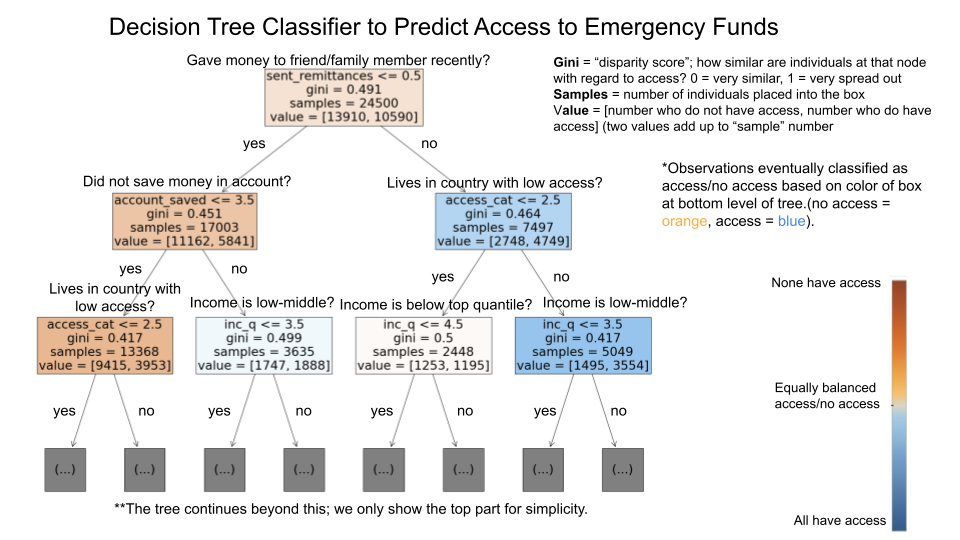
\includegraphics[width=\textwidth,height=0.5\textheight]{images/decision_tree_annotated.png}
\caption{Decision Tree Classifier Model}
\end{figure}

The decision tree model organizes the variables into a tree branching
off at each decision point based on the value of the variables at that
point. The most influential variables are at the top, and the outcome
variable is at the end of each branch. In our decision tree, the most
influential variable was sent\_remittances. Sent\_remittances is a
binary variable that asks participants, ``In the PAST 12 MONTHS, have
you, personally, GIVEN or SENT money to a relative or friend living in a
different city or area INSIDE (country where survey takes place)? This
can be money you brought yourself or sent in some other way.'' It makes
sense that this is the most influential variable in relation to access
to emergency funds, because if you have the privilege to send spare
money to loved ones, you most likely have extra money saved for yourself
as well.

Depending on the response to sent\_remittances the tree branches into
two, considering participants' responses to the next two influential
variables: access\_cat and account\_saved. Access\_cat is a variable
that categorizes the 35 sub-saharan countries by the percent of access
to emergency funds according to its participants ranging between 1-5,
with 1 being 0\%-20\% of participants in that country having access to
emergency funds, and 5 being 80\%-100\% of participants having access to
emergency funds. Depending on the country the participant lives in,
they'll be assigned to a number between 1-5 for access\_cat. On the
other hand, account\_saved is a variable that categorizes participants
based on their personal finances ranging from 1-4, with 1 representing
having no financial account and no money saved, and 4 representing
having a financial account and money saved. Being assigned 2 or 3 in
account\_saved, means you either only have a financial account, or only
have money saved, but not both.

The decision tree then splits according to participants' responses all
the way down the tree, until finally it can predict whether or not based
on the responses the participant has access to emergency funds.

\hypertarget{confusion-matrices-by-gender-figure-6}{%
\subsubsection{Confusion Matrices by Gender (Figure
6)}\label{confusion-matrices-by-gender-figure-6}}

\begin{figure}
\centering
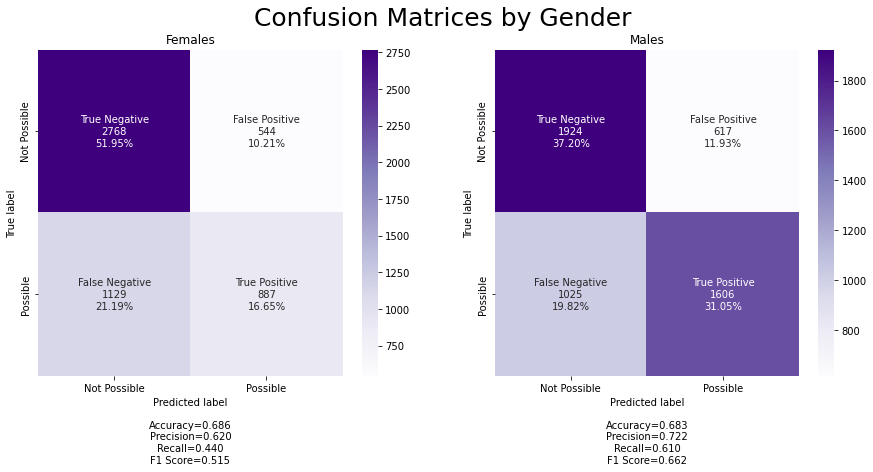
\includegraphics[width=\textwidth,height=0.5\textheight]{images/confusionMatrices.png}
\caption{Confusion Matrices by Gender}
\end{figure}

When we create two separate confusion matrices separated by gender, we
can see that the model is fairly good at predicting true negatives for
both groups, but is significantly better at predicting true positives
for males as compared to females. The false positive and false negative
error rates are also slightly higher for females as compared to males,
yet the rates are pretty similar for both models.

This may be an example of the model reinforcing biases that are present
in the data because we saw from our exploratory data analysis that many
fewer females than males have access to emergency funds, so if there are
not many females that have true positive values recorded in the data,
the model is likely to be less accurate in predicting positive outcomes
for females. This could have discriminatory impacts in the case that
this model is (hypothetically) used to determine whether or not to
provide an individual with a loan based on whether or not they have
access to emergency funds (i.e., if they do have access, they are likely
to pay back the loan, so they will get the loan, and if they do not have
access, they will not get the loan). If very few females in the training
data have access, and the model is thus less likely to predict a
positive outcome for females as we see here, this will result in fewer
females receiving loans. This will result in a self-reinforcing cycle of
continued discrimination because if the model continues to predict that
females should not get loans, fewer females will get loans, which means
fewer females would have the opportunity to pay back loans, and so on.

On the flip side, if the results of the model are (hypothetically) being
used to offer support to individuals who are in financial hardship and
do not have access to emergency funds, the accuracy in predicting
negative values would be more important, and the fact that the model is
less accurate in predicting true positives would be less of a concern.
This is because in this case, it would be a better outcome for an
individual to receive support when they do not need it (false negative)
as compared to the outcome that an individual does not receive support
when they do need it (false positive). However, we would still want the
model to be as accurate as possible on both ends in order to ensure that
we are allocating resources most directly to those who need it the most.

This comparison of confusion matrices also demonstrates the importance
of considering the balance of true negatives to true positives in
addition to just the error rates. When looking at just the error rates,
they seem almost equal between the two groups, yet when we consider the
balance of true negatives to true positives, we can see that the model
is much worse at predicting true positives for females. This furthermore
highlights the importance of trying out various methods and metrics for
assessing fairness because two different metrics can tell two completely
different stories about the degree of fairness present in the model.

\hypertarget{fairness-metrics-summary-table-figure-7}{%
\subsubsection{Fairness Metrics Summary Table (Figure
7)}\label{fairness-metrics-summary-table-figure-7}}

\begin{figure}
\centering
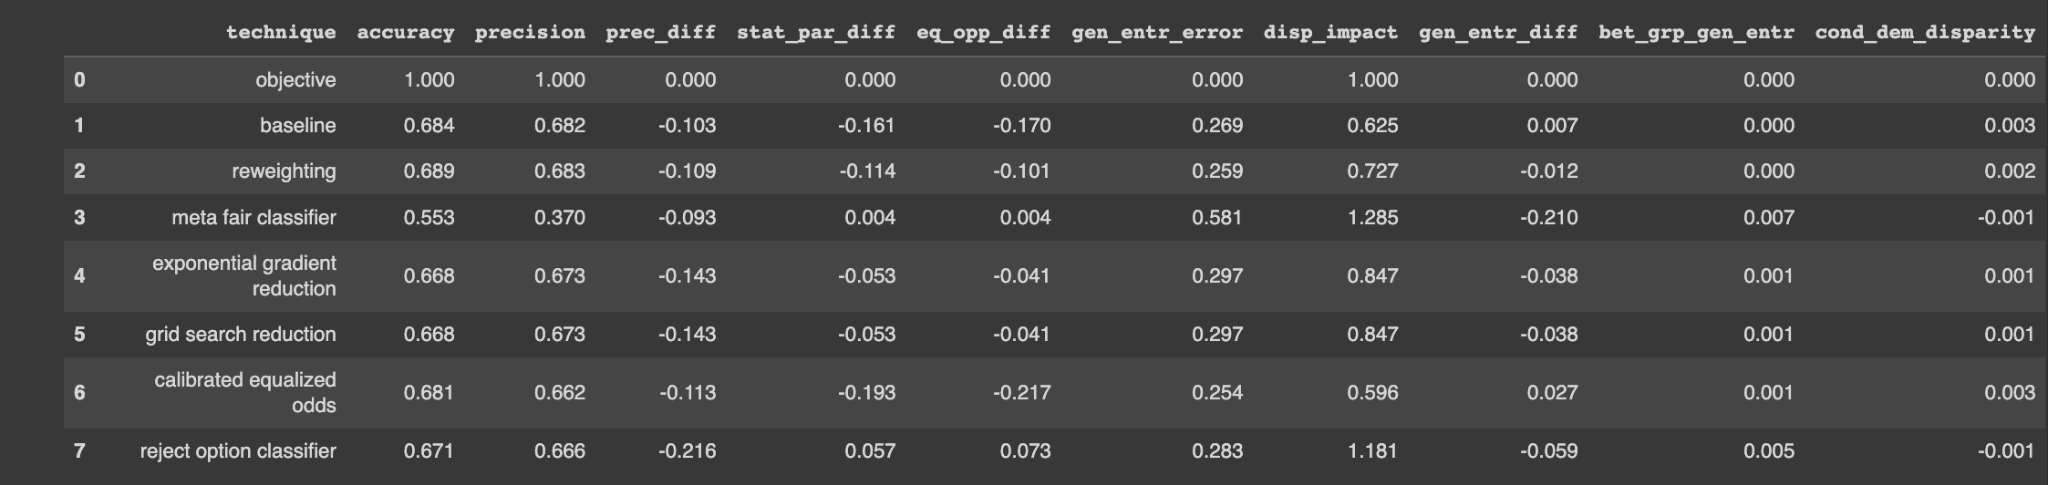
\includegraphics[width=\textwidth,height=0.4\textheight]{images/FairnessMetricsSummary.png}
\caption{Fairness Metrics Summary}
\end{figure}

Our Fairness Metrics Table compiles our Fairness Metrics and (Pre, In,
\& Post) Processing Methods that we have applied to our model. Our
metrics are seen in the columns of our table while our Processing
Techniques are in the rows. Our objective row demonstrates the ideal
ratios we would like to achieve with our Processing Techniques, while
the baseline row shows the values for our baseline model without any
processing techniques applied.

\hypertarget{baseline}{%
\paragraph{Baseline}\label{baseline}}

Our baseline model provided us with the second best model accuracy and
precision at .684 and .682. It also provided us with the closest general
entropy error difference ratio to 0, at .0007, meaning that there is
almost no difference in our Baseline model between the benefits men and
women have when it comes to having access to emergency funds.

\hypertarget{reweighting}{%
\paragraph{Reweighting}\label{reweighting}}

Our reweighting technique provided us with the highest model accuracy,
at .689, meaning that our model predicts our classifications the most
correctly when the reweighting technique is applied. Additionally, the
reweighting technique also provides us with the best ratio for
precision, at .683, indicating that applying this technique provides us
with the best model for predicting positive outcomes accurately.

\hypertarget{meta-fair-classifier}{%
\paragraph{Meta Fair Classifier}\label{meta-fair-classifier}}

The meta fair classifier provides us with an acceptable statistical
parity difference and equal opportunity difference ratio of .004 for
both, meaning that there is nearly no difference between the percentage
of females who have access to emergency funds compared to the percentage
of males who have access to emergency funds. However, because the ratio
is positive, it indicates that the model is slightly biased in favor of
women.

Both the statistical parity difference and equal opportunity difference
ratios for the meta fair classifier were at .004, which is within the
acceptable range. The statistical parity ratio indicates there is nearly
no difference between the percentage of females who have access to
emergency funds compared to the percentage of males who have access to
emergency funds. The equal opportunity difference ratio indicates that
there is nearly no difference between the accuracy in the model for
women compared to the accuracy within the model for males. However,
because these ratios are positive, they indicate that the models are
slightly biased in favor of women.

\hypertarget{exponential-gradient-reduction-grid-search-reduction}{%
\paragraph{Exponential Gradient Reduction \& Grid Search
Reduction}\label{exponential-gradient-reduction-grid-search-reduction}}

The exponential gradient reduction and grid search reduction techniques
output the same ratios for our fairness metrics. For the disparate
impact metric, we had a ratio of .847, which satisfies the acceptable
range of .80. This means that women are classified to have access to
emergency funds about 84.7\% of the time that men are categorized ro
have access to emergency funds. For our between group generalized
entropy error metric, we have ratios of .001, indicating that we have
near equal levels of inequity for our groups, meaning that we do not
have high levels of inequity between women and men at the group level.

\hypertarget{calibrated-equalized-odds}{%
\paragraph{Calibrated Equalized Odds}\label{calibrated-equalized-odds}}

Our calibrated equalized odds technique provided us a general entropy
error difference ratio of .254. A value of zero indicates that no group
benefits from our model. However, our ratio indicates that women benefit
from our model and therefore are predicted to have more false positives,
which means that women are projected to have access to emergency funds
when they in reality do not.

\hypertarget{reject-option-classifier}{%
\paragraph{Reject Option Classifier}\label{reject-option-classifier}}

The reject option classifier provides us with a ratio of -.001 for the
conditional demographic disparity metric, meaning that there is close to
an equal number of negatives and positives between our groups. However,
in our particular instance, this indicates an unfairness towards women,
since we are aware that women have less access to emergency funds
compared to men. This ratio indicates equity between our groups, which
we know is false.

\hypertarget{discussion}{%
\section{Discussion}\label{discussion}}

In this study we examine a decision tree classifier for access to
emergency funds in Sub-Saharan Africa, assess the fairness of this
classifier, use processing techniques to increase the fairness of our
model, and assess the fairness again after the processing techniques
have been applied. Our initial decision tree model is unfair towards
women in that it cannot predict true positives for women as well as it
does for men. We apply six different processing techniques and analyze
the results. We find that the processing techniques maintain most of the
accuracy and improve fairness. In our case we specifically care that the
model does not discriminate based on gender. This means we care most
about the group fairness metrics and the processors that decrease gender
discrimination in our model.

Most of the processors increased fairness for most of the fairness
metrics. The calibrated equalized odds however, decreased fairness for
all the metrics except the generalized entropy error. This would be a
good processor to use if individual fairness was a major concern in the
model. For group fairness, in our model, this processor is not ideal.

All processors besides calibrated equalized odds decreased the
statistical parity difference resulting in our model predicting more
women as having access to emergency funds. We must be careful when
interpreting this result. At first glance it may seem that these
techniques are increasing fairness, but we must consider how the other
metrics change and what this means in a real-life context. Our processed
model will classify more women as having access to emergency funds, but
this could be dangerous if these women are realistically in need of
financial support. To make sure our model is realistically being fair to
women, we must look at the processors that increase precision and equal
opportunity. Satisfying these fairness metrics would allow our model to
predict more positives for women in an accurate way.

The reweighing technique both increases precision and decreases equal
opportunity difference however, this processor only increases precision
by .1\%. None of the other processors increase precision at all. The
meta fair classifier improves the equal opportunity difference the most
out of all the processors. In fact, the ratio becomes positive meaning
that the model results in more accurately predicted women with access to
emergency funds than accurately predicted men. Only looking at equal
opportunity difference this processor seems promising, but once we
consider precision, we see a different picture. This processor decreased
our precision from 68\% to 37\%. Since precision measures the proportion
of true positives to all positives, this means we have increased our
false positives. This makes sense because if our model increases the
number of positives for women, there will be more true positives which
will satisfy our equal opportunity difference fairness metric, but there
will also be more false positives decreasing our precision.

This is a good example of how fairness can be complicated. We cannot
just look at the processor that increases fairness across the board, but
rather we must find a processor that prioritizes whatever the situation
deems as fair. In our case fairness means something different than it
would for an algorithm used in hiring practices. In a hiring scenario it
would be a good idea to predict more women as being qualified for a job
even if the false positive rate increases, because the model would be
fighting existing prejudices and give women more opportunities. In our
case fairness means something different. We want a model that classifies
women just as accurately as it does men. We focused on positive outcomes
because we decided it would be more harmful to classify someone as
having access to emergency funds when in reality they don't. This
interpretation might change depending on the context.

The equal opportunity difference is the most helpful metric in assessing
accurately predicted positives. The processors that account for the
fairness we care about are the reweighing, exponential gradient
reduction, grid search reduction, and the reject option classifier.
These these processors maintain precision while increasing positive
classifications for women.

Although these processors increase accurate positive outcomes for women,
we lose some other kinds of fairness. The generalized entropy error,
generalized entropy error difference, and between group generalized
entropy error increase when the exponential gradient reduction, grid
search reduction, and the reject option classifier processors are used.
This means that individual fairness decreases overall. The generalized
entropy error difference becomes negative meaning that men have more
generalized entropy error than women. The between group generalized
entropy error increased slightly meaning that there is more within group
unfairness than between. These results are to be expected because group
fairness and individual fairness metrics are contradictory. As we
account for group fairness, we lose individual fairness. For access to
emergency funds, we care more if our model is systematically being
unfair to women, so it is okay that we lose some individual fairness.

Our study builds from numerous other studies that developed fairness
metrics\citep{speicher2018unified, wachter2021fairness}, developed
processing
techniques\citep{agarwal2018reductions, kamiran2012data, agarwal2019fair, pleiss2017fairness},
and analyzed the trade-offs for different fairness
metrics\citep{speicher2018unified}. Where our study differs is that we
intend this study to serve as an example of how these fairness metrics
should be implemented. There must be considerations about the data, the
model, and the metrics to decide how to process the model in the
``fairest'' way. Just knowing how the different fairness metrics are
calculated is not enough. To ensure fairness one must understand how
adjusting for different fairness metrics will impact the people that the
model will be used on. If the wrong fairness metric is accounted for,
the model might reinforce social injustices.

In our study, we only looked at a decision tree classifier. For future
studies, implementing fairness metrics and processors in a specific
context on multiple different machine learning algorithms could be
helpful in seeing how these processors act for different types of
models. There are other processors and fairness metrics that were not as
applicable to our context that could be implemented in a future study.
For example, a study implementing fairness metrics in a context where
individual fairness needs to be prioritized. In our case, the model we
built was not necessarily going to be used for anything other than
educational purposes. Knowing the purpose of a model will aid in
selecting the most relevant fairness metrics and processors.

Overall, the reweighing and exponential gradient reduction techniques
are the most helpful processors for our decision tree classifier for
emergency funds in Sub-Saharan Africa. The equal opportunity difference
is the most informative fairness metric. For other models and other
contexts, this may not be true. All of these processors account for
fairness however, it is important to find the processors that account
for the specific type of fairness most relevant to the context and use
of the model.

\hypertarget{acknowledgements}{%
\section{Acknowledgements}\label{acknowledgements}}

We would like to thank our sponsor organization
\href{https://www.womenatthetable.net/}{Women at the Table}, and
especially our supervisors/mentors Sofia Kypraiou and Caitlin
Kraft-Buchman for creating the opportunity for us to do this project as
well as for offering us guidance and feedback throughout the entire
process. We would also like to thank our technical advisor, Dr.~Shiya
Cao, for providing extremely helpful Python resources and helping us
work through challenges that we were having with our code. We would like
to thank our Capstone professor, Dr.~Albert Y. Kim, for providing
conceptual and logistical guidance, especially in relation to machine
learning knowledge, as well as for providing thorough feedback on our
progress at various stages in the process. Lastly, we want to
acknowledge Megan Lyster, Assistant Director of the Smith College
Wurtele Center, for offering guidance on effective team collaboration
and helping us to continually reflect on and adapt our process as a
group throughout the course of the project.

\hypertarget{appendix}{%
\section{Appendix}\label{appendix}}

\begin{figure}
\centering
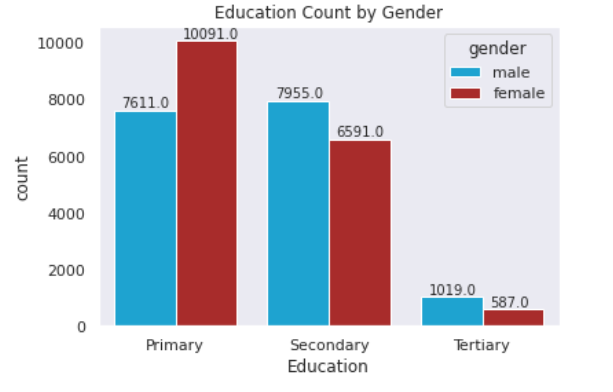
\includegraphics[width=\textwidth,height=0.5\textheight]{images/educ_count_gender.png}
\caption{Education Count by Gender}
\end{figure}

\begin{figure}
\centering
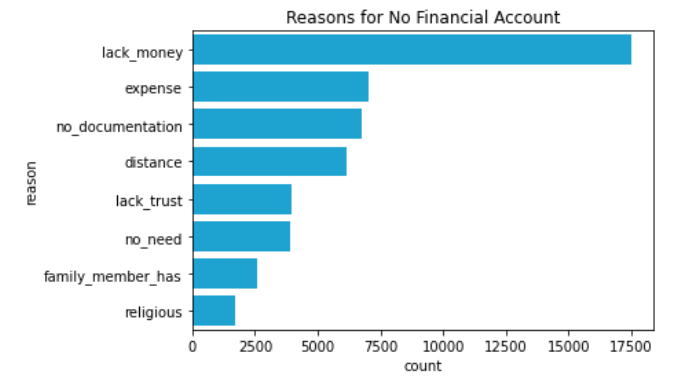
\includegraphics[width=\textwidth,height=0.5\textheight]{images/reasons_no_fin_acc.png}
\caption{Reasons for No Financial Account}
\end{figure}

% %%%%%%%%%%%%%%%%%%%%%%%%%%%%%%%%%%%%%%%%%%
% %% optional
% \supplementary{The following are available online at www.mdpi.com/link, Figure S1: title, Table S1: title, Video S1: title.}
%
% % Only for the journal Methods and Protocols:
% % If you wish to submit a video article, please do so with any other supplementary material.
% % \supplementary{The following are available at www.mdpi.com/link: Figure S1: title, Table S1: title, Video S1: title. A supporting video article is available at doi: link.}

\vspace{6pt}

%%%%%%%%%%%%%%%%%%%%%%%%%%%%%%%%%%%%%%%%%%
\acknowledgments{Project Sponsored by Women at the Table.}

%%%%%%%%%%%%%%%%%%%%%%%%%%%%%%%%%%%%%%%%%%

%%%%%%%%%%%%%%%%%%%%%%%%%%%%%%%%%%%%%%%%%%
\conflictsofinterest{The authors declare no conflict of interest.}

%%%%%%%%%%%%%%%%%%%%%%%%%%%%%%%%%%%%%%%%%%
%% optional

\input{"appendix.tex"}

%%%%%%%%%%%%%%%%%%%%%%%%%%%%%%%%%%%%%%%%%%
% Citations and References in Supplementary files are permitted provided that they also appear in the reference list here.

%=====================================
% References, variant A: internal bibliography
%=====================================
%\reftitle{References}
%\begin{thebibliography}{999}
% Reference 1
%\bibitem[Author1(year)]{ref-journal}
%Author1, T. The title of the cited article. {\em Journal Abbreviation} {\bf 2008}, {\em 10}, 142--149.
% Reference 2
%\bibitem[Author2(year)]{ref-book}
%Author2, L. The title of the cited contribution. In {\em The Book Title}; Editor1, F., Editor2, A., Eds.; Publishing House: City, Country, 2007; pp. 32--58.
%\end{thebibliography}

% The following MDPI journals use author-date citation: Arts, Econometrics, Economies, Genealogy, Humanities, IJFS, JRFM, Laws, Religions, Risks, Social Sciences. For those journals, please follow the formatting guidelines on http://www.mdpi.com/authors/references
% To cite two works by the same author: \citeauthor{ref-journal-1a} (\citeyear{ref-journal-1a}, \citeyear{ref-journal-1b}). This produces: Whittaker (1967, 1975)
% To cite two works by the same author with specific pages: \citeauthor{ref-journal-3a} (\citeyear{ref-journal-3a}, p. 328; \citeyear{ref-journal-3b}, p.475). This produces: Wong (1999, p. 328; 2000, p. 475)

%=====================================
% References, variant B: external bibliography
%=====================================
\reftitle{References}
\externalbibliography{yes}
\bibliography{mybibfile.bib}

%%%%%%%%%%%%%%%%%%%%%%%%%%%%%%%%%%%%%%%%%%
%% optional

%% for journal Sci
%\reviewreports{\\
%Reviewer 1 comments and authors’ response\\
%Reviewer 2 comments and authors’ response\\
%Reviewer 3 comments and authors’ response
%}

%%%%%%%%%%%%%%%%%%%%%%%%%%%%%%%%%%%%%%%%%%


\end{document}
